\documentclass[12pt,a4paper]{article}
\usepackage[utf8]{inputenc}
\usepackage[russian]{babel}
\usepackage[OT1]{fontenc}
\usepackage{graphicx}
\usepackage[left=1cm,right=1cm,top=1cm,bottom=1cm]{geometry}
\author{Владимир Журавлев}
\usepackage{pgfplots}
\usepackage{amsmath}
\pgfplotsset{compat=1.9}
\pagestyle{plain}
\usepackage{pgfplotstable,filecontents}

\begin{document}
\begin{flushright}
Работу выполнил:\\
\textbf{Журавлев Владимир, 621 гр.\\}
16.03 - 23.03

\end{flushright}
\begin{center}
\begin{LARGE}

\vspace{\baselineskip}
Лабораторная работа №2.4.1\\
\textbf{Определение теплоты испарения жидкости}\\
\vspace{\baselineskip}

\end{LARGE}
\end{center}

\noindent\textbf{Цель работы:} 
\begin{itemize}
\item Измерение давления насыщенного пара жидкости при разной температуре
\item Вычисление по полученным данным теплоты испарения с помощью уравнения Клапейрона-Клазиуса
\end{itemize}
\textbf{Оборудование:} термостат, герметический сосуд, заполненный исследуемой жидкостью, отсеченный микроскоп\\

\begin{Large}
\begin{center}
\textbf{1. Теория}\\
\end{center}
\end{Large}

Как известно, изотермы Ван-дер-Ваальса описываются уравнением:
\begin{equation}
(P+\frac{\alpha}{V^2})(V-b) =  RT
\end{equation}
Что соответствует графику (1).\\
\begin{minipage}{\textwidth}
        \begin{center}
        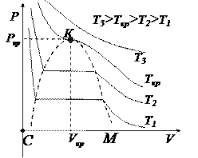
\includegraphics[scale=1]{images.png}\\
        График №1\\
        Изотермы реальных газов из уравнения \\
        Ван-дер-Ваальса\\
        \end{center}  
\end{minipage}

\noindent Проведем малый цикл Карно, совершив фазовый переход на верхней изотерме цикла. Тогда из теоремы Карно и формулы для работы:
\begin{equation}
\delta A = \delta Q_{+}\frac{dT}{T}
\end{equation}
\begin{equation} \label{maineq}
\delta A = dP (\triangle V) \Rightarrow \frac{dP}{dT} = \frac{L}{T(V_{g.}-V_{l.})}
\end{equation}
Где $V_{l.}$ и $ V_{g.} = V $ молярные объемы жидкости и газа.\\
Соответственно, достаточно измерить $\frac{dP}{dT}$, температуру и  найти молярный объем газа (объем жидкости должен вносить поправку к точности измерений ниже инструментальной)\\
Пренебрегая поправками Ван-дер-Ваальса выразим молярный объем и подставим в (\ref{maineq}), откуда получим окончательные выражения, которыми удобно оперировать:
\[V = \frac{RT}{P} \Rightarrow L = \frac{RT^2}{P} \frac{dP}{dT} = - R\frac{d(\log P)}{d(1/T)}\]
\begin{equation} \label{main}
\boxed{ L =  - R\frac{d(\log P)}{d(1/T)}}  \\
\end{equation}

\newpage
\begin{Large}
\begin{center}
\textbf{2. Экспериментальная установка}\\
\end{center}
\end{Large}
Вид установки представлен в описании работы. 
Заполненная водой ёмкость подключена
к термостату. В неё погружена запаянная ёмкость с исследуемой жидкостью;
над жидкостью находится только её насыщенный пар, давление которого
определяется по манометру при помощи отсчётного микроскопа.
Таким образом можно исследовать зависимость давления насыщенного пара
исследуемой жидкости от температуры~$P(T)$, а затем определить~$L$
с помощью~(\ref{main}).

Необходимо выдерживать скорость изменения
температуры не слишком большой, поскольку в противном случае не будет успевать
устанавливаться равновесие между теплообменной и исследуемой жидкостью, а также между
исследуемой жидкостью и её парами. В целях контроля данные измерения производятся
как при нагревании, так и при охлаждении жидкости.
Рабочее тело - спирт. Табличное значение \[L = 42.32 \; \frac{KJ}{mol} \]
Подогревание жидкости и пара происходит с помощью постоянного тока.
\begin{Large}
\begin{center}
\textbf{3. Ход работы}\\
\end{center}
\end{Large}
\paragraph{Расчет давления:} Поскольку давление пара зависит от разности показаний манометра $\Delta x = x_{1} -x_{2}$, и график для анализа работы будет построен в осях $\ln P (T^{-1})$, то важен будет только угол наклона. Поэтому расчет давления в СИ не требуется, т.к. это не изменит наклон: \[P = \rho g \Delta x \Rightarrow \ln P = \ln x + const\]
Измерим уровни ртути в манометре, а так же температуру. Результаты представлены в таблице №1.\\
Построим график $\ln \Delta x$ от $T^{-1}$.
\begin{figure}[h]
\centering
\begin{tikzpicture}
	\begin{axis}[
	 scale=1.95,
	  xlabel={$T^{-1}, K^{-1}$}, 
	  ylabel={$\ln \Delta x$},
				  domain=3.19:3.37]
		\addplot[color=blue,  mark=+, only marks] table[col sep=comma] {plot1.csv};
		\addplot[color=red,  mark=+, only marks] table[col sep=comma] {plot2.csv};
		\addplot [color = gray] {-5.1516*x + 21.177};
		\legend{Нагревание, Охлажение, МНК}
	\end{axis}
\end{tikzpicture}
\caption{График зависимости $\ln \Delta x$ от $T^{-1}$ \label{plot}}
\end{figure}

\noindentИз графика определим коэффициент наклона: $\frac{d(\ln \Delta x)}{d(T^{-1})} = -5151.6$ И получим среднее значение $L$ по формуле (\ref{main}): $L \simeq 42.81 \cdot 10^3 \frac{kJ}{mol}$\\

\paragraph{Оценка погрешностей:} приборные погрешности термометра $\Delta t = 0.1^{\circ} C$, штангенциркуля  $\Delta x = 0.1 mm$. Случайная погрешность МНК вычислена по стандартным формулам и при нагревании и охлаждении равна соответственно: $\Delta_{1} L = 0.6$ и $\Delta_{2} L = 0.7$.\\
Итоговая погрешность равна случайной, т.к. приборы не вносят значительной погрешности ($\Delta x = \frac{\Delta x}{x} \simeq 10^{-3}$, $\Delta T^{-1} = \frac{\Delta T}{T}  \simeq 10^{-4}$)\\

\begin{Large}
\begin{center}
\textbf{4. Результат}\\
\end{center}
\end{Large}
Убедившись, что приборы вносят малую погрешность в результат получим, наконец, значение $L$
\begin{Large}
\begin{equation} \label{main2}
\boxed{ L =  42.8 \pm 0.7 \; \frac{kJ}{mol}}\\
\end{equation}
\end{Large}



\begin{center}
\begin{tabular}{| c  c  c  |  c  c  c |}
\hline
$t^{o},C$&$x_{1}$, мм&$x_{2}$, мм&$\Delta x$, мм&$T^{-1}, K^{-1}$&$\ln x $\\
\hline 
24.8&32.0&81.0&49.0&3.356&3.892\\ 
25.6&31.0&81.0&50.0&3.347&3.912\\ 
26.4&29.0&83.0&54.0&3.338&3.989\\ 
26.8&28.0&83.0&55.0&3.333&4.007\\ 
27.2&28.0&84.0&56.0&3.329&4.025\\ 
27.8&27.0&86.0&59.0&3.322&4.078\\ 
28.2&26.0&87.0&61.0&3.318&4.111\\ 
30.6&22.0&89.0&67.0&3.292&4.205\\ 
31.0&22.0&90.0&68.0&3.287&4.220\\ 
31.6&20.0&92.0&72.0&3.281&4.277\\ 
32.0&20.0&93.0&73.0&3.277&4.290\\ 
32.6&18.0&94.0&76.0&3.270&4.331\\ 
33.0&17.0&95.0&78.0&3.266&4.357\\ 
33.6&16.0&96.0&80.0&3.259&4.382\\ 
34.0&15.0&98.0&83.0&3.255&4.419\\ 
34.6&14.0&99.0&85.0&3.249&4.443\\ 
35.0&13.0&99.0&86.0&3.245&4.454\\ 
35.6&11.0&102.0&91.0&3.238&4.511\\ 
36.0&10.0&102.0&92.0&3.234&4.522\\ 
36.6&8.0&104.0&96.0&3.228&4.564\\ 
37.0&8.0&105.0&97.0&3.224&4.575\\ 
37.6&7.0&105.0&98.0&3.218&4.585\\ 
38.0&6.0&108.0&102.0&3.213&4.625\\ 
38.6&4.0&109.0&105.0&3.207&4.654\\ 
39.0&3.0&109.0&106.0&3.203&4.663\\ 
39.6&0.0&111.0&111.0&3.197&4.710\\ 
39.6&1.0&110.0&109.0&3.197&4.691\\ 
39.0&2.0&108.0&106.0&3.203&4.663\\ 
38.6&3.0&108.0&105.0&3.207&4.654\\ 
38.0&4.0&107.0&103.0&3.213&4.635\\ 
37.6&7.0&106.0&99.0&3.218&4.595\\ 
37.0&8.0&106.0&98.0&3.224&4.585\\ 
36.6&8.0&104.0&96.0&3.228&4.564\\ 
36.0&10.0&101.0&91.0&3.234&4.511\\ 
35.6&11.0&100.0&89.0&3.238&4.489\\ 
35.0&13.0&93.0&80.0&3.245&4.382\\ 
34.0&14.0&97.0&83.0&3.255&4.419\\ 
33.6&15.0&96.0&81.0&3.259&4.394\\ 
33.0&17.0&95.0&78.0&3.266&4.357\\ 
32.6&18.0&93.0&75.0&3.270&4.317\\ 
32.0&20.0&92.0&72.0&3.277&4.277\\ 
27.2&28.0&84.0&56.0&3.329&4.025\\ 
26.4&29.0&82.0&53.0&3.338&3.970\\ 
\hline
\end{tabular} 

Таблица №1
\end{center}

\end{document}